\documentclass[border=3pt]{standalone}
% Preâmbulo compartilhado pelos diagramas TikZ da aula 14 (SLAM com EIF)
\usepackage[T1]{fontenc}
\usepackage[utf8]{inputenc}
\usepackage{lmodern}
\usepackage{amsmath}
\usepackage{xcolor}
\usepackage{tikz}
\usetikzlibrary{arrows.meta,angles,quotes,decorations.pathmorphing,decorations.pathreplacing,calc,
                positioning,shapes.geometric,shapes.misc,backgrounds,fit,
                math}

% Paleta (mesma dos SVGs originais)
\definecolor{dblue}{HTML}{2A5B8C}
\definecolor{dorange}{HTML}{B3541E}
\definecolor{dgreen}{HTML}{4A7C59}
\definecolor{dred}{HTML}{9C4B4B}
\definecolor{dcream}{HTML}{F4F1EA}
\definecolor{dshade}{HTML}{DDD7C9}

% Função gaussiana (não normalizada por padrão de escala visual)
\pgfmathdeclarefunction{gauss}{3}{%
  \pgfmathparse{1/(#3*sqrt(2*pi))*exp(-((#1-#2)^2)/(2*#3^2))}%
}

% Estilos comuns (prefixo d... para não colidir com chaves internas do pgf)
\tikzset{
  >={Stealth[length=2mm]},
  dguide/.style={gray!55, dashed, line width=0.4pt},
  daxis/.style={gray!60, line width=0.7pt, ->},
  dbody/.style={fill=black!3, draw=black!80, line width=1pt},
  dacc/.style={draw=dblue, line width=1pt},
  dlbl/.style={black!55, font=\small},
  dsub/.style={black!45, font=\footnotesize},
  dstate/.style={circle, draw=black!80, fill=dcream, line width=1pt,
                 minimum size=17mm, font=\large, inner sep=1pt},
  dobs/.style={circle, draw=black!80, fill=dshade, line width=1pt,
               minimum size=14mm, font=\large, inner sep=1pt},
  dbox/.style={rounded corners=2pt, draw=black!80, fill=dcream, line width=1pt,
               align=center, inner sep=6pt},
  dop/.style={circle, draw=black!80, fill=white, line width=1pt,
              minimum size=6mm, inner sep=0pt, font=\small},
  dtrans/.style={->, dblue, line width=1pt},
  dmeas/.style={->, dorange, line width=1pt},
  dcurve/.style={line width=1pt, dblue},
  dcurveb/.style={line width=1.4pt, dorange},
}

\begin{document}
\hyphenpenalty=10000 \exhyphenpenalty=10000 \tolerance=9999 \emergencystretch=3em
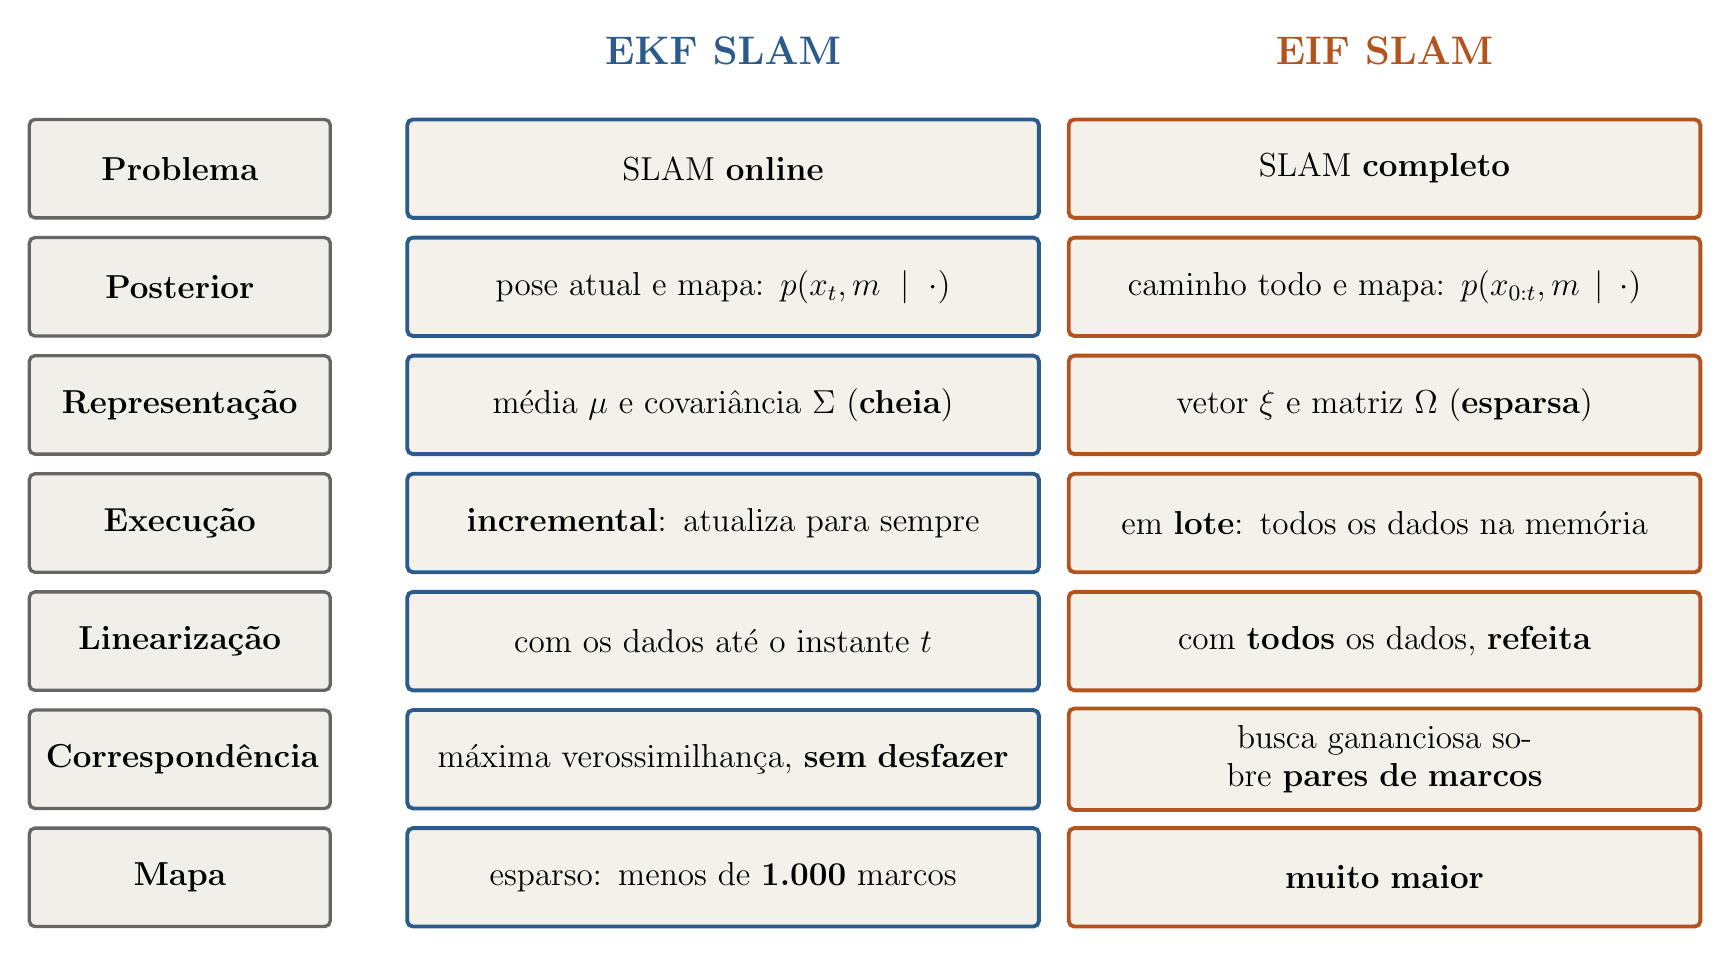
\begin{tikzpicture}[x=1cm,y=1cm]
\node[font=\Large\bfseries, text=dblue] at (8.8,9.9) {EKF SLAM};
\node[font=\Large\bfseries, text=dorange] at (17.2,9.9) {EIF SLAM};
\node[dbox, draw=black!60, text width=3.4cm, minimum height=1.25cm, font=\large\bfseries, line width=1.2pt, fill=dshade!40] at (1.9,8.4) {Problema};\node[dbox, draw=dblue, text width=7.6cm, minimum height=1.25cm, font=\large, line width=1.4pt] at (8.8,8.4) {SLAM \textbf{online}};\node[dbox, draw=dorange, text width=7.6cm, minimum height=1.25cm, font=\large, line width=1.4pt] at (17.2,8.4) {SLAM \textbf{completo}};
\node[dbox, draw=black!60, text width=3.4cm, minimum height=1.25cm, font=\large\bfseries, line width=1.2pt, fill=dshade!40] at (1.9,6.9) {Posterior};\node[dbox, draw=dblue, text width=7.6cm, minimum height=1.25cm, font=\large, line width=1.4pt] at (8.8,6.9) {pose atual e mapa: $p(x_t,m\mid\cdot)$};\node[dbox, draw=dorange, text width=7.6cm, minimum height=1.25cm, font=\large, line width=1.4pt] at (17.2,6.9) {caminho todo e mapa: $p(x_{0:t},m\mid\cdot)$};
\node[dbox, draw=black!60, text width=3.4cm, minimum height=1.25cm, font=\large\bfseries, line width=1.2pt, fill=dshade!40] at (1.9,5.4) {Representação};\node[dbox, draw=dblue, text width=7.6cm, minimum height=1.25cm, font=\large, line width=1.4pt] at (8.8,5.4) {média $\mu$ e covariância $\Sigma$ (\textbf{cheia})};\node[dbox, draw=dorange, text width=7.6cm, minimum height=1.25cm, font=\large, line width=1.4pt] at (17.2,5.4) {vetor $\xi$ e matriz $\Omega$ (\textbf{esparsa})};
\node[dbox, draw=black!60, text width=3.4cm, minimum height=1.25cm, font=\large\bfseries, line width=1.2pt, fill=dshade!40] at (1.9,3.9) {Execução};\node[dbox, draw=dblue, text width=7.6cm, minimum height=1.25cm, font=\large, line width=1.4pt] at (8.8,3.9) {\textbf{incremental}: atualiza para sempre};\node[dbox, draw=dorange, text width=7.6cm, minimum height=1.25cm, font=\large, line width=1.4pt] at (17.2,3.9) {em \textbf{lote}: todos os dados na memória};
\node[dbox, draw=black!60, text width=3.4cm, minimum height=1.25cm, font=\large\bfseries, line width=1.2pt, fill=dshade!40] at (1.9,2.4) {Linearização};\node[dbox, draw=dblue, text width=7.6cm, minimum height=1.25cm, font=\large, line width=1.4pt] at (8.8,2.4) {com os dados até o instante $t$};\node[dbox, draw=dorange, text width=7.6cm, minimum height=1.25cm, font=\large, line width=1.4pt] at (17.2,2.4) {com \textbf{todos} os dados, \textbf{refeita}};
\node[dbox, draw=black!60, text width=3.4cm, minimum height=1.25cm, font=\large\bfseries, line width=1.2pt, fill=dshade!40] at (1.9,0.9) {Correspondência};\node[dbox, draw=dblue, text width=7.6cm, minimum height=1.25cm, font=\large, line width=1.4pt] at (8.8,0.9) {máxima verossimilhança, \textbf{sem desfazer}};\node[dbox, draw=dorange, text width=7.6cm, minimum height=1.25cm, font=\large, line width=1.4pt] at (17.2,0.9) {busca gananciosa sobre \textbf{pares de marcos}};
\node[dbox, draw=black!60, text width=3.4cm, minimum height=1.25cm, font=\large\bfseries, line width=1.2pt, fill=dshade!40] at (1.9,-0.6) {Mapa};\node[dbox, draw=dblue, text width=7.6cm, minimum height=1.25cm, font=\large, line width=1.4pt] at (8.8,-0.6) {esparso: menos de \textbf{1.000} marcos};\node[dbox, draw=dorange, text width=7.6cm, minimum height=1.25cm, font=\large, line width=1.4pt] at (17.2,-0.6) {\textbf{muito maior}};
\end{tikzpicture}
\end{document}
